\documentclass[parskip=half]{scrartcl}

\usepackage{xcolor}
\usepackage{hyperref}
\hypersetup{
    colorlinks,
    linkcolor={red!50!black},
    citecolor={blue!50!black},
    urlcolor={blue!80!black}
}

\usepackage{graphicx}
\graphicspath{ {./images/} }

\usepackage{microtype}
\usepackage{fontspec}

\newcommand\figref{Figure~\ref}

\let\oldFootnote\footnote
\newcommand\nextToken\relax

\renewcommand\footnote[1]{%
    \oldFootnote{#1}\futurelet\nextToken\isFootnote}

\newcommand\isFootnote{%
    \ifx\footnote\nextToken\textsuperscript{,}\fi}

\usepackage[
    backend=biber,
    style=ieee,
]{biblatex}
\addbibresource{ref.bib}

\setmainfont{Georgia}
\setsansfont{Helvetica Neue}

\KOMAoptions{DIV=calc}

\begin{document}

\input{../author}

\begin{center}
    \Large
    \textsf{\textbf{Open-Source Intelligence}}
        
    \vspace{0.4cm}
    \large
    Homework 2: Privacy Preserving Technologies
        
    \vspace{0.4cm}
    \docauthor{}
       
    \vspace{0.9cm}
\end{center}

\tableofcontents

\section{Preamble}

My pseudonym for the course is \textit{raccoon dog}. \figref{fig:og_img} shows
the image assigned to me.

\begin{figure}[h]
\includegraphics[width=\textwidth]{raccoon dog}
\centering
\caption{\texttt{raccoon dog.jpg}}
\label{fig:og_img}
\end{figure}

We see that we are dealing with a ship, and a cargo ship for that matter. This
is good news, as there should be plenty of official information regarding the
ship available online.

\section{Photo Summary}

\begin{itemize}
    \item Photographer: Bernard Spragg
    \item Source: \url{https://www.flickr.com/photos/volvob12b/28237039302}
    \item Date taken: July 14, 2016 at 16:21 UTC+12
    \item Camera model: Panasonic DMC-FZ1000
    \item Approximate camera price: 688 € (July 2016, Estonia)
    \item Photographer ``level'': enthusiast
    \item Photo location: Lyttleton Harbor, Lyttleton, New Zealand
    \item Photo subject: OOCL Dalian Cargo Ship (HK)
    \item Approximate temperature: 12°C
\end{itemize}

\section{Detailed Steps}

\subsection{Locating the Image Source}

The first thing I attempted was to search for the ship's name on Google Images.
I was in luck, since searching for \textit{OOCL Dalian} yields this exact image
among the first results. Additionally, the image can also be found by Google
Images reverse search.

The image was uploaded to Flickr\footnotemark by Bernard Spragg. The image being
available on Flickr is good news, because some important EXIF image metadata is
automatically displayed on the site, so there is no need for extra tooling such
as \texttt{exiftool}.
\footnotetext{\url{https://www.flickr.com/photos/volvob12b/28237039302}}

For good measure, I downloaded the original image from Flickr and compared its
hash with the hash of the image provided by the lecturer. The hashes matched, so
I presume that the provided image has not been tampered with. Hash comparison
should be reliable here, because EXIF metadata is baked into the image data,
unlike OS/filesystem metadata. Therefore, changing EXIF metadata should change
the file's hash value.

\subsection{Establishing the Capture Time}

From the metadata, the image was captured on July 14, 2016. While the capture
time is reported as 16:21:00+00:00 by the image's EXIF, which would mean that
the time is UTC time, which seems a little suspicious. In July, New Zealand
observes New Zealand Standard Time (NZST) which is UTC+12. As such, it would
have been 04:21 local time at the picture's capture time, which would most
likely not match the lighting conditions.

Cameras are however often configured with local time, and so they assume local
time as UTC time, if the time zone is not or cannot additionally be configured.
Moreover, the local time zone assumption seems to be confirmed by another piece
of metadata---the metadata date field---which was most likely given by the
photo processing software, and which gives the time 21:45:22+12:00, thus
confirming the NZST timezone. We can hence conclude that the image was captured
on July 14, 2016, at 16:21 UTC+12.

According to historical weather data\footnotemark, the temperature in the area
at the time of capture was around 54°F which is about 12.22°C, without
precipitations, and with good visibility. There is nothing on the picture that
would indicate that this these measurements are significantly off, so the
temperature seems plausible. This temperature also seems to fit with the
average temperatures in New Zealand during July~\cite{temperature}.

\footnotetext{\url{https://www.wunderground.com/history/daily/nz/diamond-harbour/NZCH/date/2016-7-14}}

However, these measurements were measured by the Christchurch International
Airport Station, and hence are not completely accurate to the location. While
there seems to be a station much closer by, i.e., the  Diamond Harbour-Purau
Station\footnotemark, there does not seem to be historical data available from
that station in particular.

\footnotetext{\url{https://www.wunderground.com/weather/nz/diamond-harbour/IDIAMO4}}

I could not recover historical weather data from the MetService---New Zealand's
national weather authority~\cite{metservice}---for that time period
either, neither from their website, nor from the Wayback Machine\footnotemark.

\footnotetext{\url{https://web.archive.org/web/20160801000000*/https://www.metservice.com/towns-cities/regions/christchurch/locations/eastern-suburbs}}

\subsection{Geolocating the Capture Point}

By using \texttt{exiftool}, it does not seem that the GPS coordinates of where
the image was taken are part of the metadata. On Flickr however, the author has
marked the location where there image was captured on a map.

By opening the map, from the URL bar we can extract the coordinates
\begin{center}
    Lat$=-43.613148$, Lon=$172.731084$
\end{center}
which translate to $43$°$36$'$47.3$"S $172$°$43$'$51.9$"E. The coordinates refer
to a point in the channel between Lyttleton Port and Diamond Harbour in
Lyttleton, New Zealand. \figref{fig:gmaps_sat} shows a screenshot from Google
Maps with a pin on the found coordinates.

\begin{figure}[ht]
    \includegraphics[width=\textwidth]{gmaps_sat}
    \centering
    \caption{Google Maps location}
    \label{fig:gmaps_sat}
\end{figure}

It would be logical that the coordinates mark the approximate location of the
camera, and not of the ship itself. We can attempt to confirm this using Google
Street View.

Unfortunately, due to the location, Street View is a little lacking, with
available locations shown on \figref{fig:streetview_spots}. Still, we can try to
approximate the angle of the photographer relative to the target based on a
geographic landmarks---the path of woods on a hill---circled in red on
\figref{fig:streetview_spots}.

\begin{figure}[ht]
    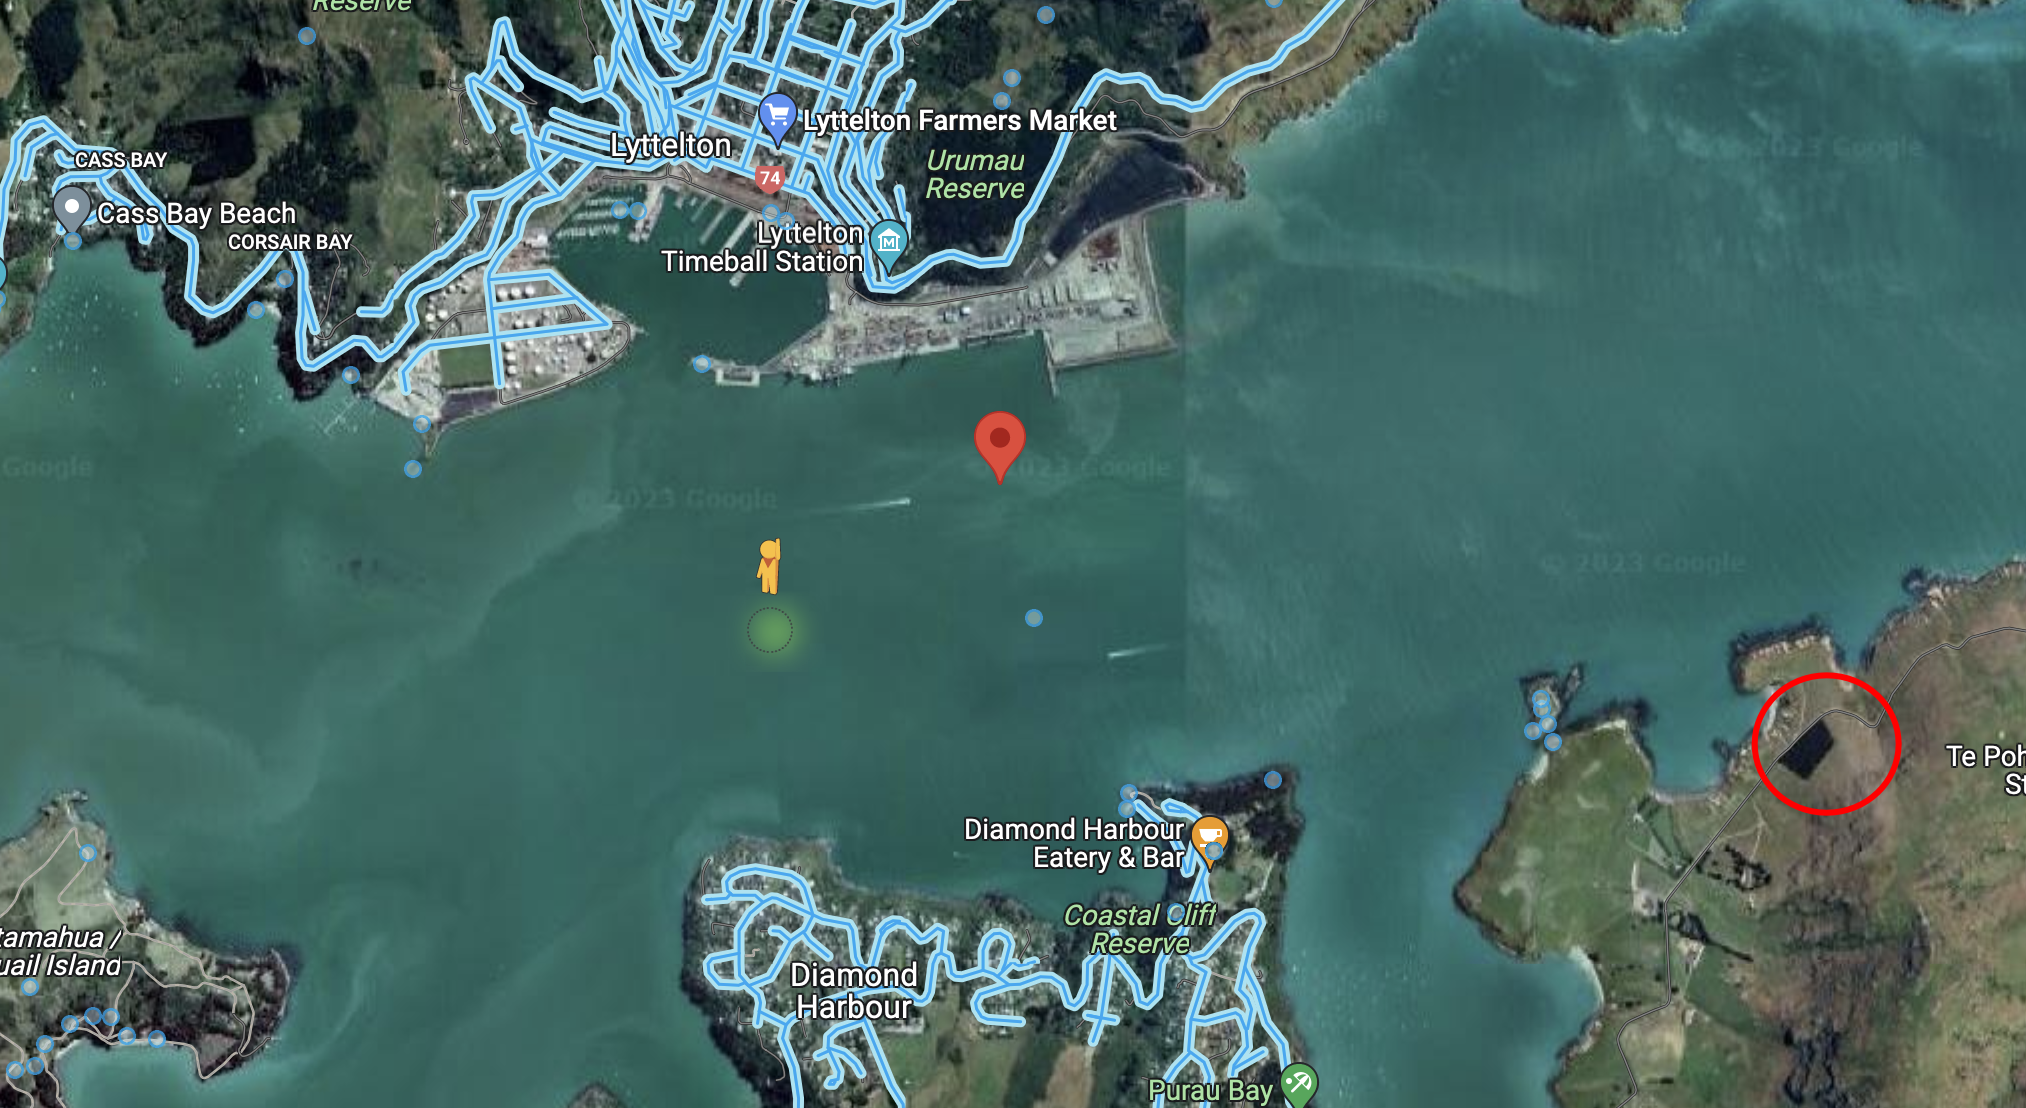
\includegraphics[width=\textwidth]{maps1-marked}
    \centering
    \caption{Google Maps street view spots}
    \label{fig:streetview_spots}
\end{figure}

\figref{fig:streetview_anno1} is the street view from the location in water
closest to the red position marker in Google Maps, oriented towards the
landmark, and zoomed in. While the resolution is not that great, i.e., we cannot
clearly see the horizontal cliff pattern on the leftmost mountain, we can see
that the angles are fairly close (but not exact) compared to the original image.

\begin{figure}[ht]
    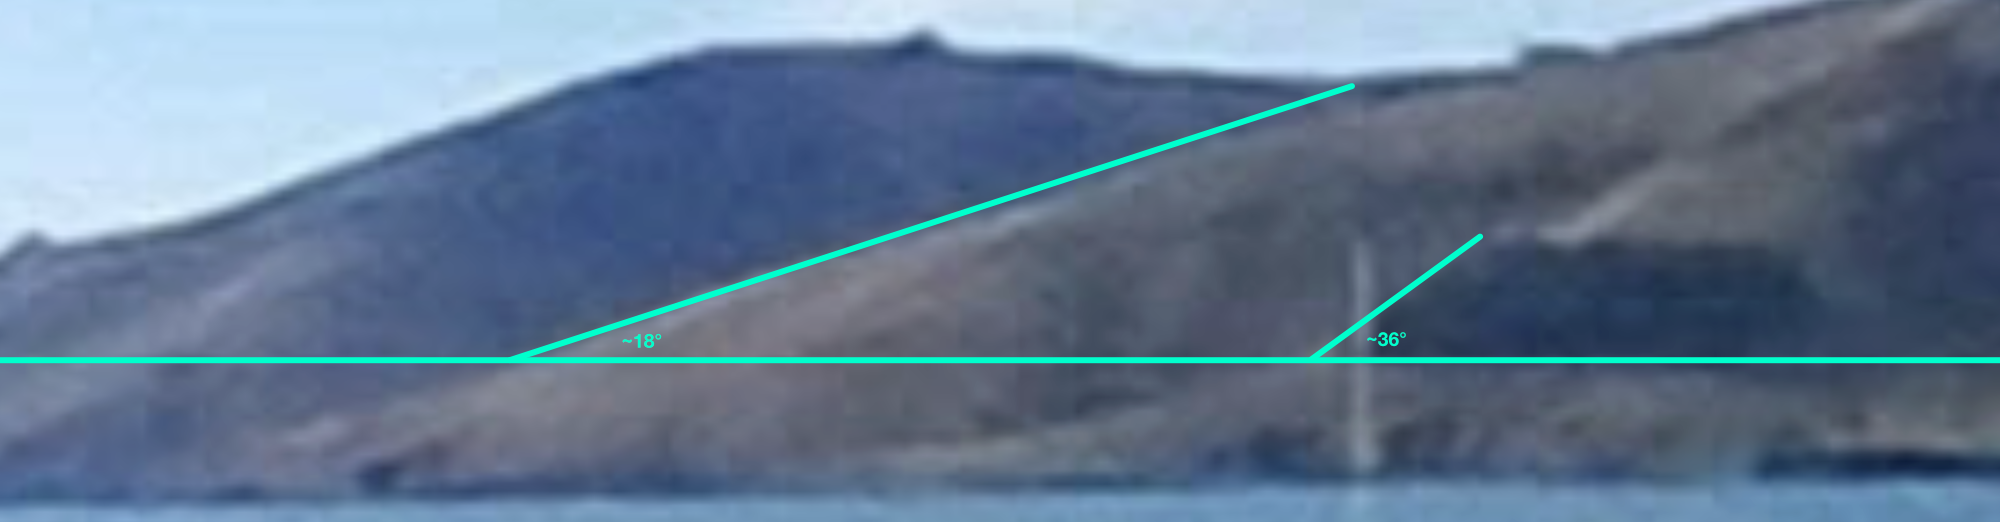
\includegraphics[width=\textwidth]{sv_ss1_annotated}
    \centering
    \caption{Street view of the landmark}
    \label{fig:streetview_anno1}
\end{figure}

A street view upload from Pony Point---an area slightly to the left of Cass Bay
Beach but outside the area of \figref{fig:streetview_spots}---gives us a better
look to the geographic landmarks, as shown on \figref{fig:streetview_anno2}.
Moreover, this street view picture was captured in August 2016, so roughly in
the month following the capture of the original picture, guaranteeing the
``freshness'' of the landmarks. \figref{fig:los} shows the line of sight of the
street view in \figref{fig:streetview_spots}.

\begin{figure}[ht]
    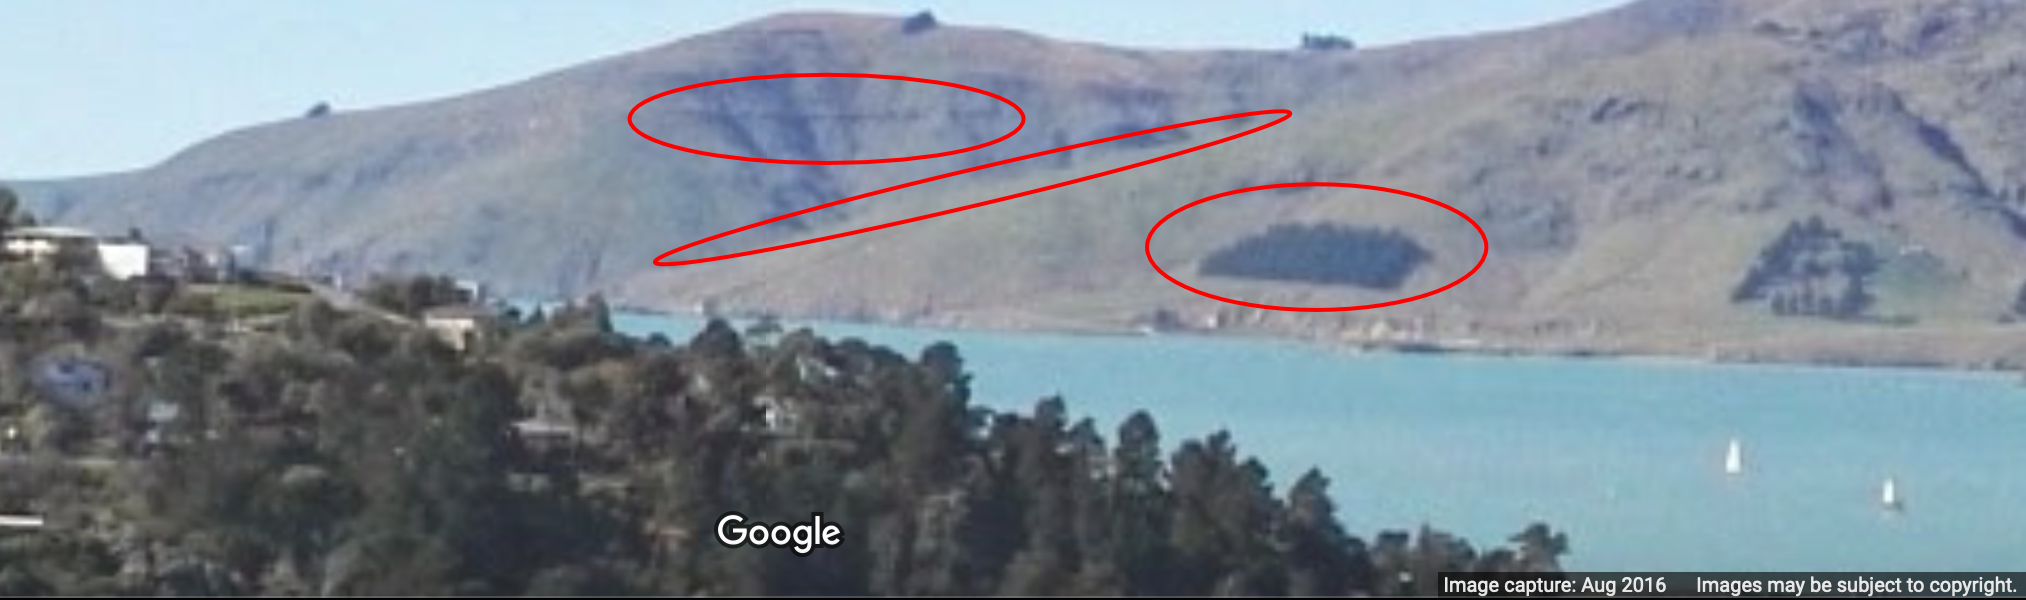
\includegraphics[width=\textwidth]{sv_ss2_annotated}
    \centering
    \caption{Landmarks in August 2016}
    \label{fig:streetview_anno2}
\end{figure}

\begin{figure}[ht]
    \includegraphics[width=\textwidth]{los}
    \centering
    \caption{Line of sight from the source of \figref{fig:streetview_anno2}}
    \label{fig:los}
\end{figure}

It seems hence safe to say that the location coordinates roughly do match the
approximate location of the camera. It could probably be feasible to narrow the
location down better using some calculations, but this seems out of scope for
the given assignment.

As for the location of the ship itself, while this too could be calculated
based on the camera's zoom/field of vision, and the ship's length and relative
position against the background, such precise calculations are out of scope for
the given task. \figref{fig:shiploc} shows the area where the approximate area
where the ship could have been at the image capture time. The approximate
coordinates are then 43°36'51.9"S 172°44'42.9"E (the centre of the red
ellipse).

\begin{figure}[ht]
    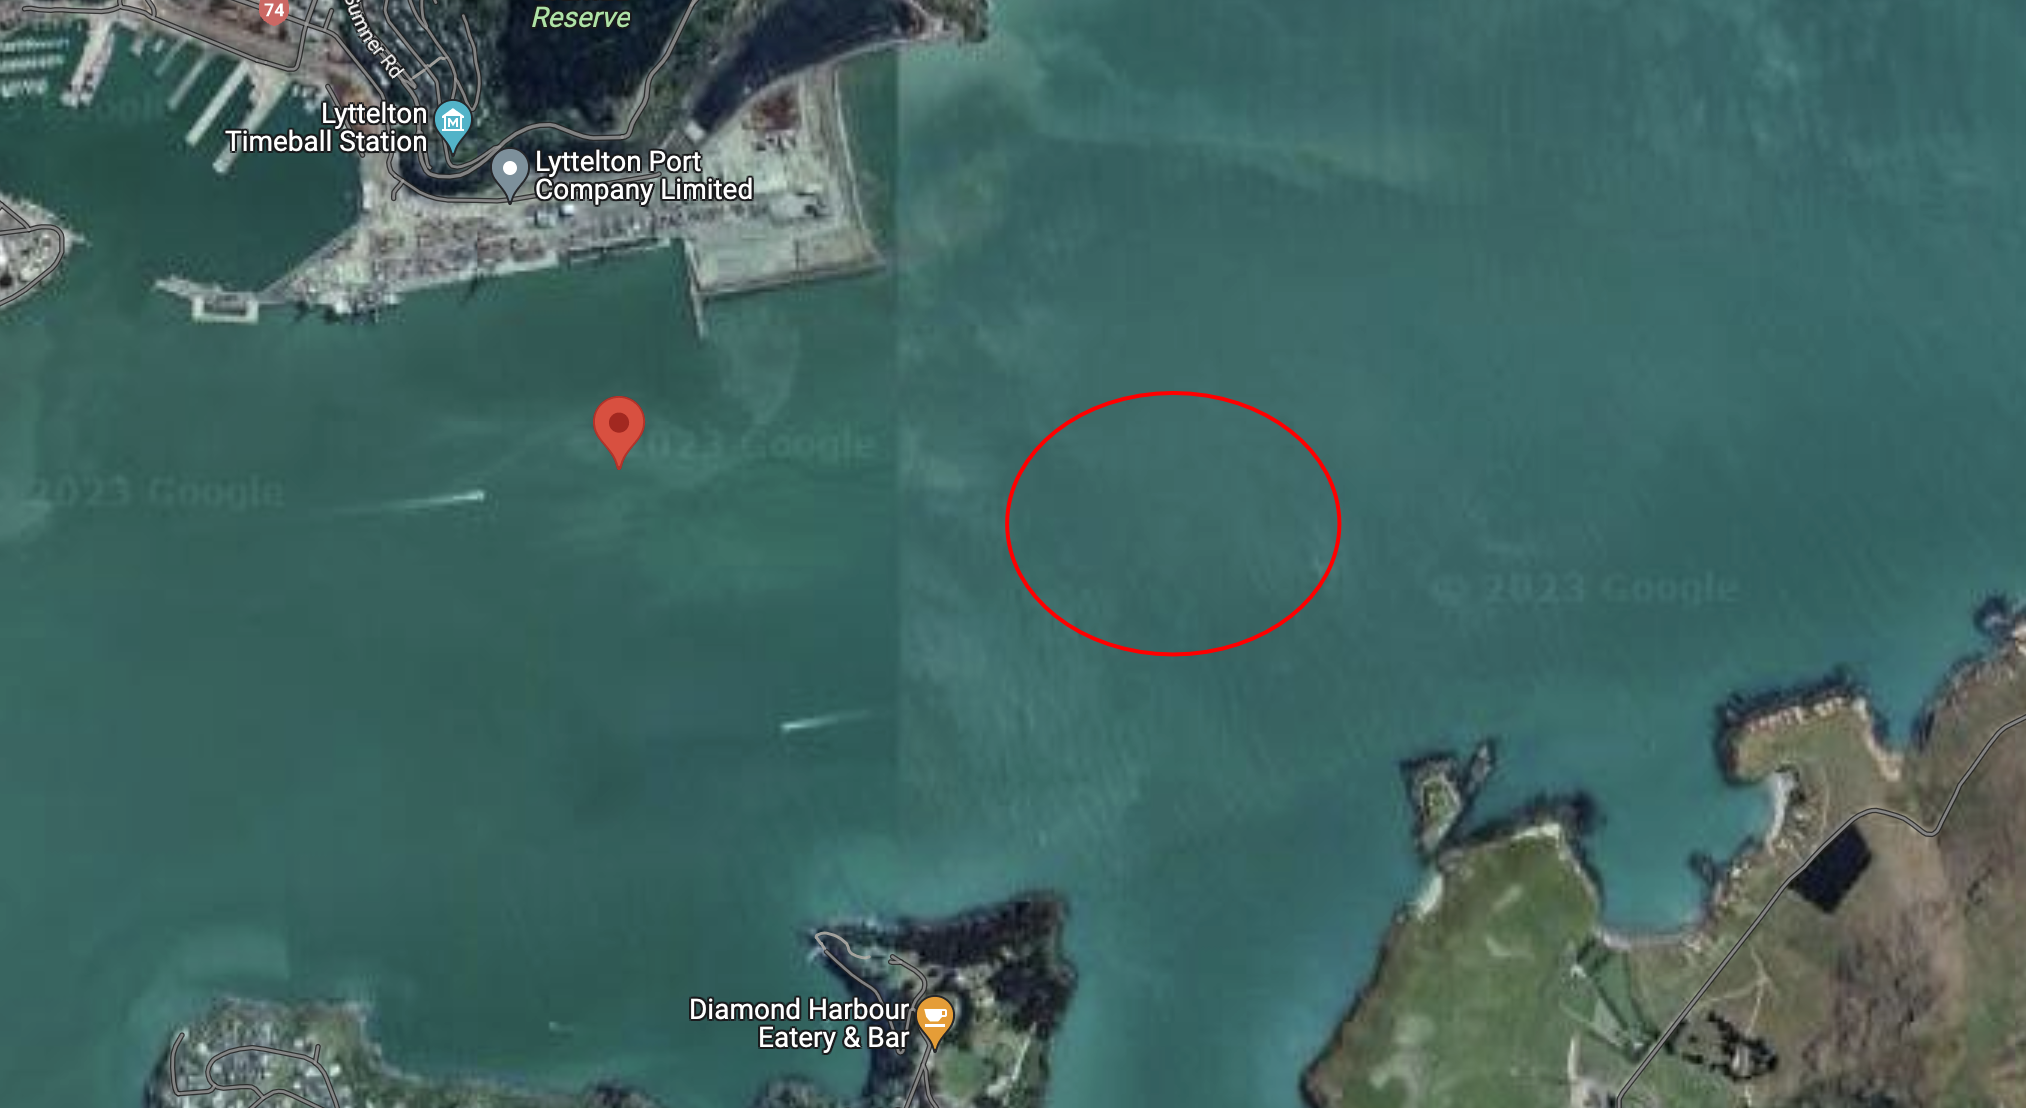
\includegraphics[width=\textwidth]{shiploc}
    \centering
    \caption{Approximate location of the picture subject}
    \label{fig:shiploc}
\end{figure}

\iffalse
By looking at the initial picture, it is clear that the coordinates cannot mark
the location of the OOCL Dalian, but the coordinates may be of the spot the
picture was taken from.
\fi

% https://www.flickr.com/photos/volvob12b/52592447201/in/photostream/

\subsection{Camera Details}

The model of the camera is marked in the EXIF metadata of the picture. The photo
was taken with a Panasonic DMC-FZ1000 on July 14, 2016. To find the price of the
camera at the time, I have to do some digging.

I initially attempted to find the price history by browsing some NZ
sites\footnote{\url{https://www.priceme.co.nz}}\footnote{\url{https://pricespy.co.nz}}
but those only had prices for the Panasonic Lumix DMC-FZ1000 II released in
2019. The original DMC-FZ1000 was released in 2014 \cite{prnewswire}.

Therefore, to get some idea of the price of the original camera in July 2016, I
ended up using the Estonian Hinnavaatlus\footnotemark website to look up the
lowest price in Estonia around the date the picture was taken. The closest
available data point (before the capture date) is of July 11, 2016, and the
cheapest price in Estonia for the camera at the time was 688 €.
\figref{fig:hinnavaatlus} displays a section of the price evolution graph.
\footnotetext{\url{https://hinnavaatlus.ee}}

\begin{figure}[ht]
    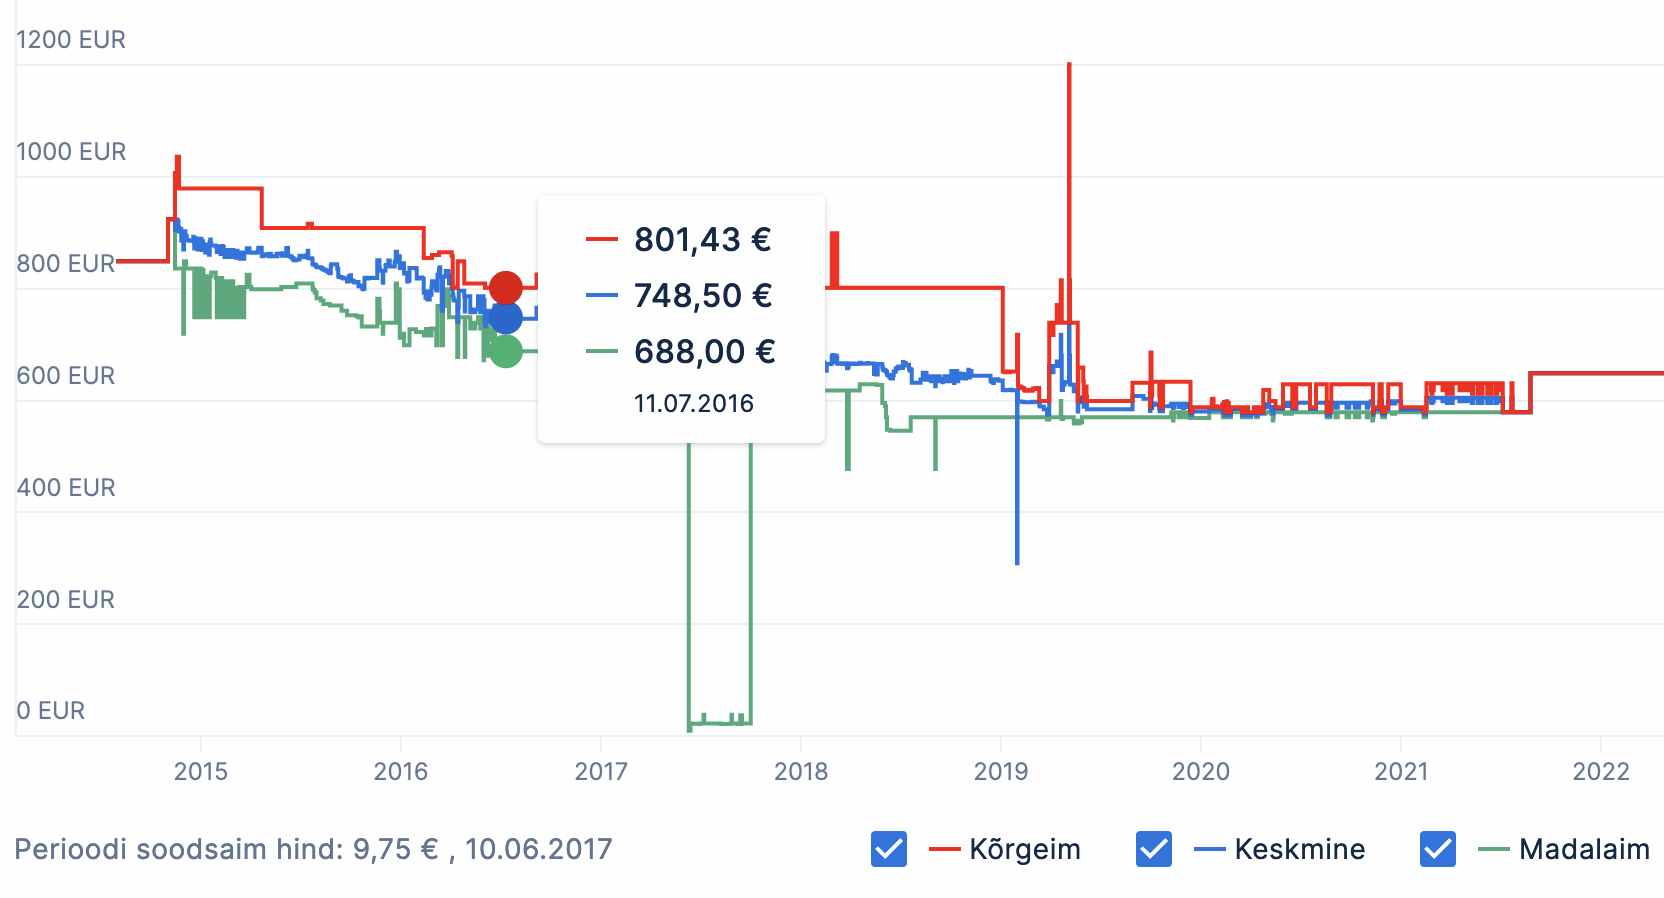
\includegraphics[width=\textwidth]{hinnavaatlus}
    \centering
    \caption{Historic price from \texttt{hinnavaatlus.ee}}
    \label{fig:hinnavaatlus}
\end{figure}

By looking at the camera's spec sheet\footnotemark and considering its price, it
seems to me that the photographer is not a professional, but is an involved
hobbyist, i.e., not a complete beginner.
\footnotetext{\url{https://www.panasonic.com/mea/en/consumer/cameras-camcorders/lumix-digital-cameras/dmc-fz1000.specs.html}}

One reason that leads me to believe that the photographer is not a professional
is that the lens of the camera is not interchangeable, and not ``at the level''
of a professional's fixed lens of choice. The picture's subjective quality and
the price of the camera lead me to believe that the photographer has some
interest and skill in photography, and hence is likely an enthusiast.

The photographer's Flickr portfolio and description of themselves seem to
support my guess.

\subsection{Subject Details}

Finding information about the subject---OOCL Dalian---was trivial. It sufficed
to type in the ship's name into a search engine. Some of the more interesting
results are:
\begin{itemize}
    \item ​OOCL Dalian's
    \href{https://www.oocl.com/eng/ourservices/vessels/pclass4500/Pages/oocldalian.aspx}
    {general characteristics} on \texttt{oocl.com}
    \item OOCL Dalian's
    \href{https://www.marinetraffic.com/en/ais/details/ships/shipid:688458/mmsi:477627800/imo:9445526/vessel:OOCL_DALIAN}
    {current and historic location} on \texttt{marinetraffic.com}
\end{itemize}

OOCL Dalian was built in 2009, has the call sign VRFW9, is registered in Hong
Kong and its International Ship Security Certificate expires in
2025~\cite{oocldalian}.

Information about the location is just as easily accessible, since the location
is known.

\printbibliography[heading=bibintoc]

\end{document}
